%\documentclass[trans,handout]{beamer}
\documentclass[trans]{beamer}

%\usepackage{pgfpages}
%\pgfpagesuselayout{4 on 1}[a4paper,landscape,border shrink=5mm]
%\pgfpagesuselayout{2 on 1}[a4paper,border shrink=5mm]

\usepackage[utf8]{inputenc}
\usepackage{graphicx}
\usepackage{multicol}
\usepackage{xcolor}
\usepackage{listings}
\lstset{frame=tb,
  aboveskip=3mm,
  belowskip=3mm,
  showstringspaces=false,
  columns=flexible,
  basicstyle={\small\ttfamily},
  numbers=none,
  numberstyle=\tiny\color{gray},
  keywordstyle=\color{blue},
  commentstyle=\color{green!55!blue},
  stringstyle=\color{purple},
  breaklines=true,
  breakatwhitespace=true,
  tabsize=4
}
\usepackage{hyperref}
\hypersetup{
  colorlinks=true,
  linkcolor=black,
  urlcolor=blue
}
\graphicspath{{figures/}}

\title{
  
\includegraphics[height=.2\textheight]{../figures/biopython.jpg}\\[1em]
  Biopython Project Update 2017}
\subtitle{}
\author[Sourav Singh]{
  \textbf{Sourav Singh}, Christian Brueffer, Peter Cock,\\
  and the Biopython Contributors}
\institute[University of Pune]{University of Pune\\
  India\\[1em]
  Bioinformatics Open Source Conference 2017, Prague, CZ \\[1em]
}
\date{July 23th, 2017}


\setcounter{tocdepth}{2}
\setbeamertemplate{caption}{\insertcaption}


% ToC at the beginning of every section
%\AtBeginSection[]
%{
 % \begin{frame} % with <beamer> => doesn't appear in handout mode
  %  \frametitle{Outline} %% Put the title you want, or none!
  %  \tableofcontents[currentsection,currentsection]
 % \end{frame}
%}

\begin{document}
\maketitle

\section{The Biopython Project}
\frame
{
  \frametitle{What is Biopython?}

  \begin{itemize}
  \item Collection of modules for biological computation in Python
  \begin{itemize}
  \item Sequence handling and motifs, parsers, database queries, protein structures, phylogenetics, tool wrappers and more.
  \end{itemize}
  \item Started in 1999, first release in 2000
  \item Open source and freely available (Biopython license)
  \end{itemize}

  \begin{center}
  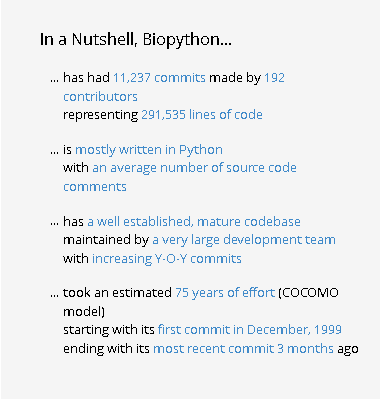
\includegraphics[width=0.4\textwidth]{figures/openhub-bp-nutshell.png}
  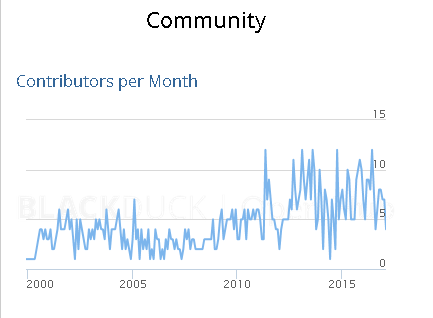
\includegraphics[width=0.5\textwidth]{figures/openhub-bp-community-activity.png}
  \end{center}
  \small{Source: \url{https://www.openhub.net/p/biopython}}
}
\frame
{
  \frametitle{Lots of new contributors!}

  \scriptsize{
  \begin{multicols}{3}
  \begin{itemize}
  %1.68
  \item Anthony Bradley
  \item Ben Fulton
  \item Carlos Pena
  \item Connor T Skennerton
  \item Iddo Friedberg
  \item Kai Blin
  \item Kristian Davidsen
  \item Markus Piotrowski
  \item Olivier Morelle
  \item Peter Cock
  \item Stefans Mezulis
  \item Tiago Antao
  \item Travis Wrightsman
  \item Uwe Schmitt
  \item Xiaoyu Zhuo

  %1.69
  \item Adam Kurkiewicz
  \item Adam Novak
  \item Adrian Altenhoff
  \item Allis Tauri
  \item Andrew Guy
  \item Andrew Sczesnak
  \item Blaise Li
  \item Brandon Carter
  \item Foen Peng
  \item Francesco Gastaldello
  \item Francisco Pina-Martins
  \item Hector Martinez
  \item Jack Twilley
  \item Jeroen Van Goey
  \item Joshua Meyers
  \item Kurt Graff
  \item Leonhard Heizinger
  \item Marcin Magnus
  \item Maximilian Greil
  \item Michał J. Gajda
  \item Milind Luthra
  \item Oscar G. Garcia
  \item Richard Neher
  \item Sourav Singh
  \item Spencer Bliven
  \item Steve Marshall
  \item Veronika Berman
  \end{itemize}
  \end{multicols}
  }
}

%%%%%%%%%%%%%%%%%%%%%%%%%%%%%%%%%%%%%%%%%%%%%%%%%%%%%%%%%%%%%%%%%%%%%%%%%%%%%%%%

\section{New Releases and Beyond}
\frame
{
\center{\LARGE Biopython 1.68(released 2016-08-25)}
}
\frame
{
  \frametitle{New Features in Biopython 1.68}

  \begin{itemize}
  \item Final Release supporting Python 2.6
  \item Added extension to \texttt{Bio.PDB} to allow for parsing of the new MMTF format. Requires
  \item \texttt{Bio.pairwise2} rewritten to address speed and problems with local alignments.
  \item \texttt{SeqGui} and \texttt{xbbtools} rewritten using tkinter.
  \item Biopython now uses HTTPS instead of HTTP to connect to Entrez and QBLAST API.
  \end{itemize}

}
\frame
{
  \center{\LARGE Biopython 1.69 (released 2017-04-06)}
}
\frame
{
  \frametitle{Start of re-licensing plan}

  \begin{itemize}
  \item 1.69 marks the start of start of our re-licensing plan, to transition away
from liberal \emph{Biopython License Agreement} to the widely used \emph{3-Clause BSD License}.
\item The code base-authorship is being reviewed file-by-file, in order to gradually dual license the entire
project.
  \end{itemize}

}

\frame
{
  \frametitle{New parser for ExPASy cell line database}

  \begin{itemize}
  \item \texttt{Bio.ExPASy}:
  \begin{itemize}
  \item Cellosaurus cell line database, cell ontologies and cell line catalogues.
  \item Now accessible through the \texttt{Bio.ExPASy} module.
  \end{itemize}
  \end{itemize}
}
\frame
{
  \frametitle{Other new features to Biopython 1.69}
  \begin{itemize}
  \item MAF files are now supported using the \texttt{Bio.AlignIO.MafIO} module
  \item Also offers indexed access for large files using SQLite3.
  \item Update to \texttt{Bio.Restriction} to include REBASE February 2017 restriction enzyme list.
  \item \texttt{Bio.PDB.PDBList} can download PDBx/mmCif (new default), PDB (old default), PDBML/XML and MMTF format protein structures.
  \item \texttt{Bio.Affy} module supports version 4 of Affymetrix CEL format\
  \end{itemize}

}


\frame
{
  \frametitle{Miscellaneous}

  \begin{itemize}
  \item Miscellaneous bug fixes
  \item Test suite enhancements
  \item Better PEP8 and PEP257 coding style adherence
  \item Enhanced PyPy support by taking
advantage of NumPy and compiling most of the Biopython C code modules
  \end{itemize}
}


\subsection*{Current Developments}
\frame
{
  \center{\LARGE What's cooking for Biopython 1.70?}
}


\frame
{
  \frametitle{Biopython 1.70-dev}

  \begin{itemize}
  \item Module \texttt{Bio.AlignIO}
  \begin{itemize}
  \item Support for XMFA file format.
  \item using Bio.AlignIO.MauveIO
  \end{itemize}
  \end{itemize}
  \begin{itemize}
  \item Module \texttt{Bio.SearchIO}
  \begin{itemize}
  \item Support for new arguments to read and write blast-xml files.
  \end{itemize}
  \item Drop support for Python 3.3
  \end{itemize}

}
\frame
{
  \frametitle{New logo for Biopython}

  \begin{itemize}
  \item Version 1.70 marks the transition towards a new logo for Biopython.

  \begin{center}
  
\includegraphics[width=0.5\textwidth]{figures/biopython_logo_s.png}
  \end{center}

  \item The new logo was created by Patrick Kunzmann in 2017 and had support from Python Software Foundation and the Biopython developers community.
  \end{itemize}

}
\frame
{
  \frametitle{Supported Python Versions}

  \begin{itemize}
  \item Python 2.7
  \item Python 3.4
  \item Python 3.5
  \item PyPy 5.0
  \item PyPy3 2.4
  \item Jython 2.7
  \end{itemize}
}

\section{General Updates}
\frame
{
  \frametitle{Continuous Integration}

  \begin{itemize}
  \item TravisCI
  \item Experimentation with Build Stages for CI testing.
  \begin{itemize}
  \item Codecov.io (test coverage)
  \item Quantified Code (metrics and automatic pull requests)
  \item Landscape.io (``health score'')
  \end{itemize}
  \item Currently enabled by default: Codecov.io, Quantified Code
  \end{itemize}

  \begin{columns}
  \column{0.4\textwidth}
  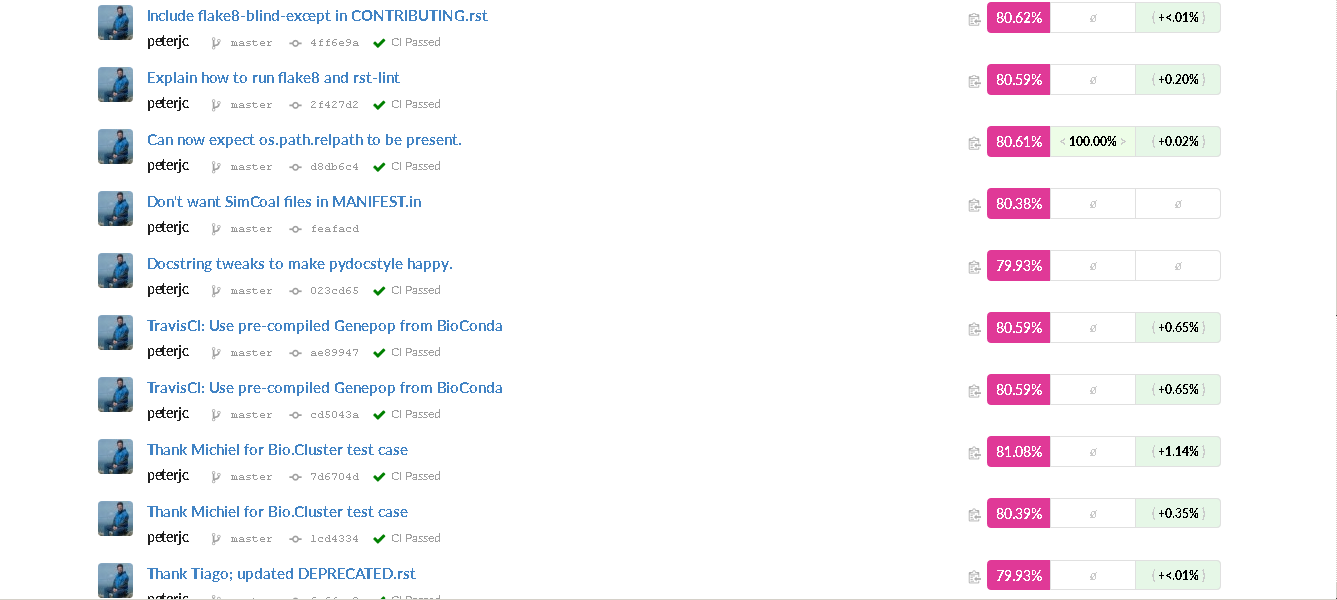
\includegraphics[width=1\textwidth]{figures/bp-codecov.png}
  \column{0.6\textwidth}
  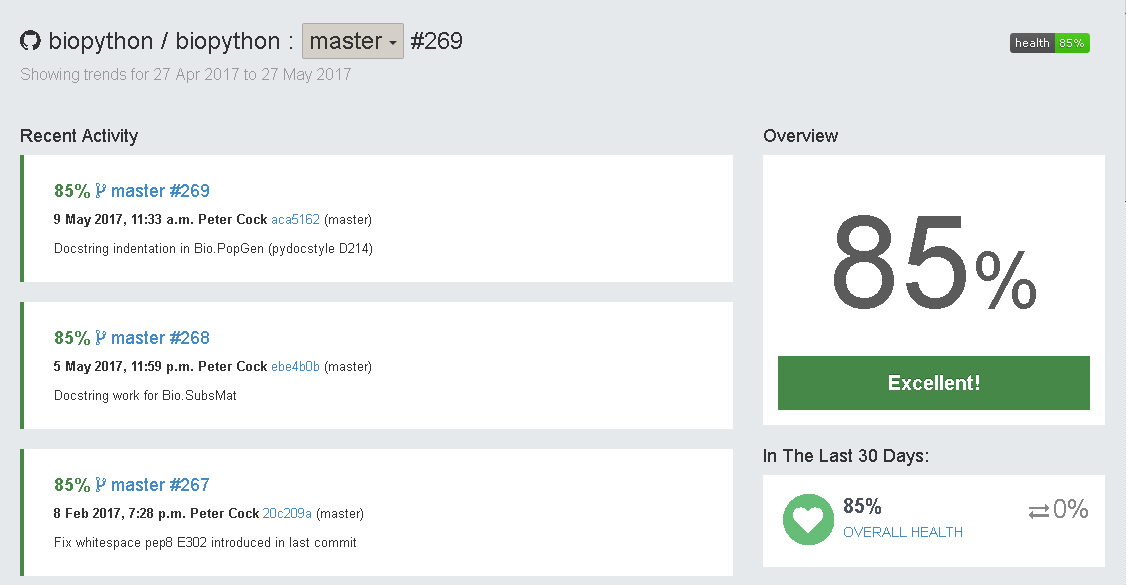
\includegraphics[width=1\textwidth]{figures/bp-landscape.png}
  \end{columns}
}

\section{Conclusion}
\frame
{
  \frametitle{Conclusion}

  \begin{itemize}
  \item Lots of new contributors
  \item Lots of new stuff
  \item Turn new contributors into recurring ones
  \item Biopython 1.70 in the near future
  \end{itemize}
}

\frame
{
  \frametitle{Acknowledgements}

  \begin{minipage}{1\textwidth}
  \begin{columns}
  \column{0.5\textwidth}
  \begin{itemize}
  \item Peter Cock
  \item Biopython Community
  \end{itemize}
  \column{0.5\textwidth}
  
\includegraphics[width=0.8\textwidth]{figures/biopython.jpg}
  \end{columns}
  \end{minipage}

  \vspace{0.5cm}

  \begin{minipage}{1\textwidth}
  \begin{columns}
  \column{0.2\textwidth}
  
\includegraphics[width=0.5\textwidth]{figures/github-logo.jpg}
  \column{0.2\textwidth}
  
\includegraphics[width=0.5\textwidth]{figures/travisci-logo.png}
  \column{0.2\textwidth}
  
\includegraphics[width=0.5\textwidth]{figures/codecov-logo.png}
  \column{0.2\textwidth}
  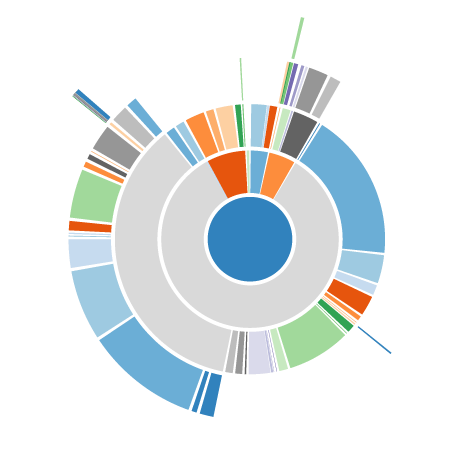
\includegraphics[width=0.5\textwidth]{figures/quantifiedcode-logo.png}
  \column{0.2\textwidth}
  
\includegraphics[width=0.5\textwidth]{figures/obf-logo.png}
  \end{columns}
  \end{minipage}
}

\section*{Acknowledgements}
\frame
{
  \frametitle{Resources!}

  %\begin{center}
  Website:\\
  \begin{itemize}
  \item \url{http://biopython.org}
  \end{itemize}

  Repositories:\\
  \begin{itemize}
  \item Main: \url{http://github.com/biopython/biopython}
  \item Website: \url{https://github.com/biopython/biopython.github.io}
  \end{itemize}

  Mailing lists:
  \begin{itemize}
  \item General list: \url{biopython@biopython.org}
  \item Developers list: \url{biopython-dev@biopython.org}
  \end{itemize}

  Biostars:
  \begin{itemize}
  \item \url{https://www.biostars.org/t/biopython/} (``biopython'' category)
  \end{itemize}
  %\end{center}
}

\end{document}
